% LTeX: enabled=true

\chapter{Commande hybride}
\minitoc


\section{Motivation}
Basée sur les capacités d'un \textit{tailsitter}, il est légitime de se poser la question du mode de vol utilise pour rejoindre un point. Effectivement, le drone a la possibilité de se déplacer en stationnaire ou bien en vol d'avancement. Lors d'un déplacement en stationnaire, le drone est vertical donc il se retrouve fortement sujet aux perturbations. Il est donc nécessaire d'avoir une grande région d'attraction autours de la position d'équilibre pour assurer un rejet des perturbations et une stabilisation.

Nous avons donc proposé une stratégie de commande pour stabiliser le drone en position stationnaire. Cette stratégie repose sur une dynamique discrète permettant le passage d'une loi de commande non-linéaire présenté dans \cite{2020e-MicCenZacFra} et qui fournit une grande région d'attraction et une seconde loi basée sur la dynamique linéarisée et fournissant une agressivité supérieure pour réaliser l'approche finale. Les deux contrôleurs sont réunis par un mécanisme hybride qui permet de conserver les performances en régime permanent de la conception linéarisée avec la grande région d'attraction garantie par la conception non linéaire. Notre solution est testée en simulant le modèle non linéaire complet.

Nous allons nous concentré dans cette partie à la stabilisation stationnaire du drone ainsi nous nous appuyrons sur la dynamique simplifier décrite dans la section \ref{sec:model_NL_simp} avec la simplification $\boldsymbol{w} = 0$ qui permet d'obtenir la dynamique simplifier sans vent \eqref{eq:withouwind}. 



\subsection{Contrôleur par retour d'état non-linéaire}
Nous illustrons dans cette section une loi de contrôle dynamique non linéaire inspirée du résultat de \cite{2020e-MicCenZacFra}. Pour que cette loi de contrôle non linéaire soit applicable, les matrices $F$ et $M$ mentionné dans \eqref{eq:withouwind} doit permettre de définir une direction dite de moment zéro $\boldsymbol{\bar u} \in \real^4$ garantissant
$|F\boldsymbol{\bar u}| = 1$ et $M \boldsymbol{\bar u}=0$, et la matrice inverse à droite $M^r$ de $M$ satisfaisant $M M^r = I$ et $FM^r=0$. Dans notre cas, il est immédiat de voir que la direction du moment zéro $\boldsymbol{\bar u} = \frac{\sqrt{2}}{2a_{\text{f}}}\smallmat{1&1&0&0}^\top$ satisfait les conditions, alors que le fait que $\rank(F) = 2$ (donc que le noyau de $F$ ($\ker F$) est de dimension 2) rend impossible l'obtention de la matrice inverse à droite $M^r$ de $M$ entièrement contenu dans $\ker F$.

En raison de cela, nous déterminons $M^r$ en paramétrisant (de manière conservatrice) les pseudoinverses droites de $M$ comme $M^r := KM^\top ( MKM^\top)^{-1}$ où la matrice $K \in \real^{4\times 4}$ est symétrique et satisfait $MKM^\top \geq I$ (pour assurer l'invertibilité). Avec cette paramétrisation, le but est de minimiser la norme de $FM^r = F KM^\top ( MKM^\top)^{-1}$, ce qui est bien réalisé en minimisant la norme de $F KM^\top$, du fait que la contrainte sur $MKM^\top \geq I$ garantissant que le facteur $( MKM^\top)^{-1}$ a une norme plus petite que 1.

% Performing a Schur complement, this minimization is well obtained by solving the following semi-definite program:
% \begin{align*}
% &  \min_{K, \kappa} \kappa, \; \mbox{subject to:}
% \;  M K M^\top\! \geq \!I, \; 
%   \begin{bmatrix}
%   \kappa I  &\! F K M^\top \\ 
%    M K^\top F^\top &\! \kappa I
%   \end{bmatrix}\! \geq\! 0,
% \end{align*}
% which minimizes $\kappa$ while ensuring $F K M^\top M K^\top F^\top \leq \kappa^2 I$. Solving this optimization, we obtain, for the specific matrices under consideration,
% \begin{align*}
%   K \!=\! \smallmat{  0   &   -737   &    171   &   -171\\
%       -737  &  0   &  -171  &     171\\
%        171  &    -171    &   1583.5    &   -43.73\\
%       -171  &     171    &   -43.73    &   1583.5}\!, \,
%   M^r \!=\! \smallmat{0     &          0   &   -3.19\\
%                  0      &         0   &    3.19\\
%                -4.51    &  -27.75    &   -1.48\\
%                 4.51    &  -27.75    &    1.48}
% \end{align*}
% leading to $\kappa = 39.7$. With this optimality-based selection, the nonlinear dynamic design of \cite{2020e-MicCenZacFra} can be effectively applied by obtaining responses that are almost indistinguishable from the fully decoupled case 
% $FM^r=0$. Note that a similar approach, essentially neglecting the extra terms acting on the translational dynamics is also suggested in the survey paper \cite{hamel_minhduc}. 

% Based on the above-described choice of $M^r$ and $\boldsymbol{\bar u}$, applying the feedback law in \cite[eqn (19)]{2020e-MicCenZacFra}, the input $\boldsymbol{u}$ becomes : 
% \begin{align}
% \label{eq:u_nonlin}
%     \boldsymbol{u} = \boldsymbol{u_{\text{nl}}} := M^r \boldsymbol{\tau_{r}} + \boldsymbol{\bar u} \boldsymbol{f},
% \end{align}
% where $\boldsymbol{\tau_{r}}$ and $\boldsymbol{f}$ are provided by the dynamic feedback controller proposed in \cite{2020e-MicCenZacFra}.

% The optimality-based selection of $M^r$ is prone to a few interesting interpretations when observing the product 
% $M^r \boldsymbol{\tau_{r}} = M^r \smallmat{\tau_{r,x} & \tau_{r,y} & \tau_{r,z}}^\top$. First, 
% % Three observations can be made. Indeed, we observe that 
% to produce a moment $\tau_{r,z}$ about the $z$-axis we mainly use the thrust differential action; secondly, a moment $\tau_{r,y}$ about the $y$-axis is generated by an equal (additive) use of the two flaps, with great efficiency; finally a moment $\tau_{r,x}$ about the $x$-axis comes from a differential use of the flaps. 

% As a final remark, as compared to the solution proposed in \cite{2020e-MicCenZacFra}, to partially take into account the saturation effects highlighted in Remark~\ref{rem:saturation}, the error feedback interconnection of the outer loop in \cite{2020e-MicCenZacFra} has been augmented with a simple error governor strategy never allowing the translational position error $\boldsymbol{\rm e}_p$ 
% entering \cite[eqn. (22)]{2020e-MicCenZacFra} to exceed the maximum value of 3 meters. 
% The remaining tuning gains required in the solution of \cite{2020e-MicCenZacFra} have been selected
% following an intuitive PD tuning procedure
%  as  $k_{pp} = 0.5$, $k_{pd} = 1.2$, $k_{ap} = 0.08$, $k_{ad} = 0.1$ and $k_{\Delta} = 1$.
 
% Figure~\ref{fig_global_contol} shows the response of the system in terms of linear and angular positions (top two rows) and actuators efforts (bottom two rows) when the system starts from the initial condition  $\boldsymbol{x(0)} = [\boldsymbol{p(0)}~ \boldsymbol{v(0)}~ \boldsymbol{q(0)}~ \boldsymbol{\omega_b(0)}]^\top = [0~0~0 ~ 0~0~0 ~0.9140 ~0.1134~ -0.3728~ 0.1134~ 0~ 0~ 0]^\top $ with a target equilibrium position of $\boldsymbol{p_{\text{eq}}} = [4~5~6]^\top$ and $\boldsymbol{q_{\text{eq}}} = [\frac{\sqrt{2}}{2}~0~-\frac{\sqrt{2}}{2}~0]^\top$. 
% % (this is associated to a large initial error of ??????? ).
% A graceful response can be seen, which remains quite far from the actuator saturations (see Remark~\ref{rem:saturation}). Increasing the tuning gains can speed up the response but provides undesired attitude oscillations. Therefore it is interesting to combine this nonlinear controller (providing a large region of attraction) with a more aggressive controller, designed based on the linearized dynamics \eqref{eq:linearized} and to be used to improve the fail of the response.
% \begin{figure}[ht!]
%     \centering
%     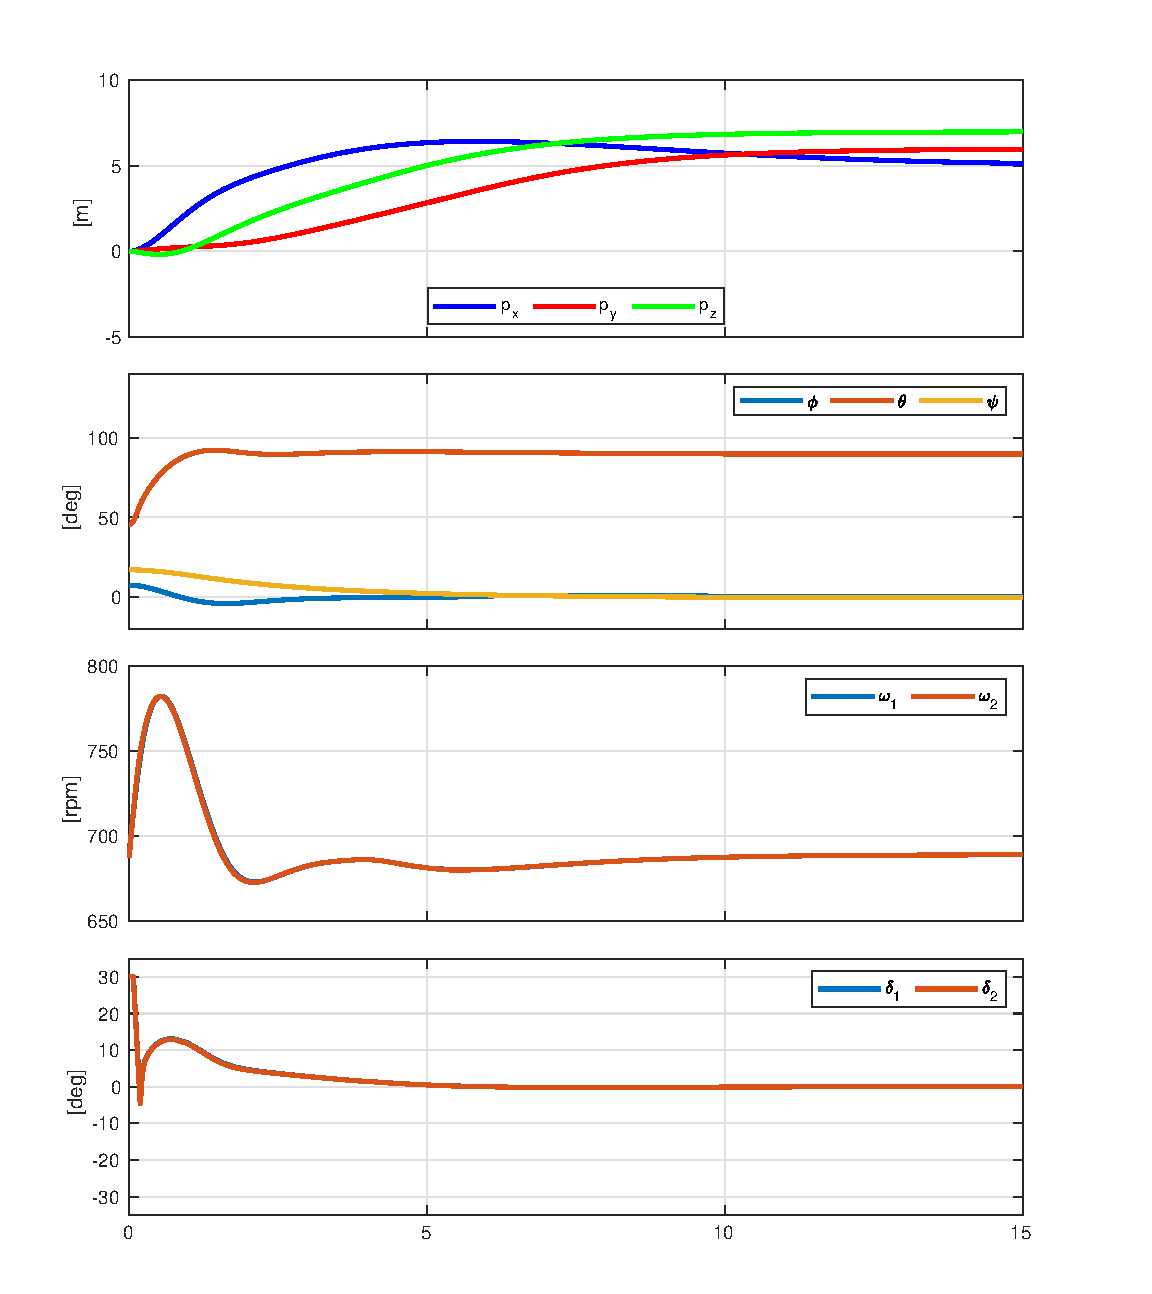
\includegraphics[trim=0cm 0.6cm 0cm 0.6cm,clip,width=1\columnwidth, height=7cm]{figures/global2.eps}
%     \vspace*{-6mm}
%     \caption{Simulation with the nonlinear dynamic feedback controller.}
%     \label{fig_global_contol}
% \end{figure}
% \subsection{Linear control design}

% Based on the performance-oriented observations of the previous section, given a target position corresponding to an equilibrium $\boldsymbol{p_{\text{eq}}}, \boldsymbol{q_{\text{eq}}}$ as characterized in Proposition~\ref{prop:eqs}, we design here a local linear feedback controller capable of inducing a more aggressive response. To this end, we focus on the linearized dynamics \eqref{eq:linearized} and recognize that we can design 
% a state feedback controller 
% \begin{align}
%   \boldsymbol{u_{\text{lin}}} := \boldsymbol{u_{\text{eq}}} - K \boldsymbol{\tilde x},
% \label{eq:u_lin}
% \end{align}
% where $\boldsymbol{\tilde x}$ has been introduced in \eqref{eq:xtilde} and $K \in \real^{4 \times 12}$ is a state feedback gain that can be designed, based on the matrices $A$ and $G$ appearing in \eqref{eq:linearized}, in such a way that the closed-loop linear feedback $A_{\text{cl}}:=A-GK$ be exponentially stable. 

% For our design, we have used an LQR selection, associated with the simplest possible weight matrices selection $Q = I_{12}$ and $R = I_{4}$, which gives desirable closed-loop responses. The LQR design also provides a positive definite Lyapunov certificate matrix $S \in \real^{12 \times 12}$ (solution of the algebraic Riccati equation) ensuring that $A_{\text{cl}}^\top S + S A_{\text{cl}} <0$. In particular, it is well known from the linear approximation theorem that function $V(\boldsymbol{\tilde x}) = \boldsymbol{\tilde x}^\top S \boldsymbol{\tilde x}$ is also a Lyapunov function certifying local exponential stability of $\boldsymbol{x_{\rm eq}}$ for the nonlinear dynamics. More specifically, there exits a positive scalar $\bar v \in \real$ such that, along dynamics \eqref{eq:dyna_simp}, we have :
% \begin{align}
% \label{eq:Vdecrease}
%   V(\boldsymbol{\tilde x}) \leq \bar v \quad \Rightarrow \quad \dot V(\boldsymbol{\tilde x}) := \langle 
% \nabla V(\boldsymbol{\tilde x}), \boldsymbol{\dot{\tilde x}}\rangle <0,
% \end{align}
% for all $\boldsymbol{\tilde x} \neq 0$; in other words, the sublevel set $V(\boldsymbol{\tilde x}) \leq \bar v$ is contained in the basin of attraction of the equilibrium $\boldsymbol{x_{\text{eq}}}$.
 
% Determining the largest possible scalar $\bar v$ ensuring \eqref{eq:Vdecrease} is a challenging problem and conservative lower bounds of this quantity can be determined by quantifying the effect of the nonlinearities on the dynamics. Since $\boldsymbol{\dot{\tilde x}}$ is a function of $\boldsymbol{x}$, then it is fairly easy to algebraically evaluate $\dot V(\boldsymbol{\tilde x})$ for a large amount of random extractions of the variable $\boldsymbol{\tilde x}$, so as to get a probabilistic estimate of the largest $\bar v$. Rigorous guarantees about these selections can be obtained by applying the results in \cite{tempo2013randomized}, which is out of the scope of this paper, but an evaluation of 10000 samples confirmed that the value $\bar v = 400$  is a good candidate selection satisfying \eqref{eq:Vdecrease}.

% \begin{figure}[ht!]
%     \centering
%     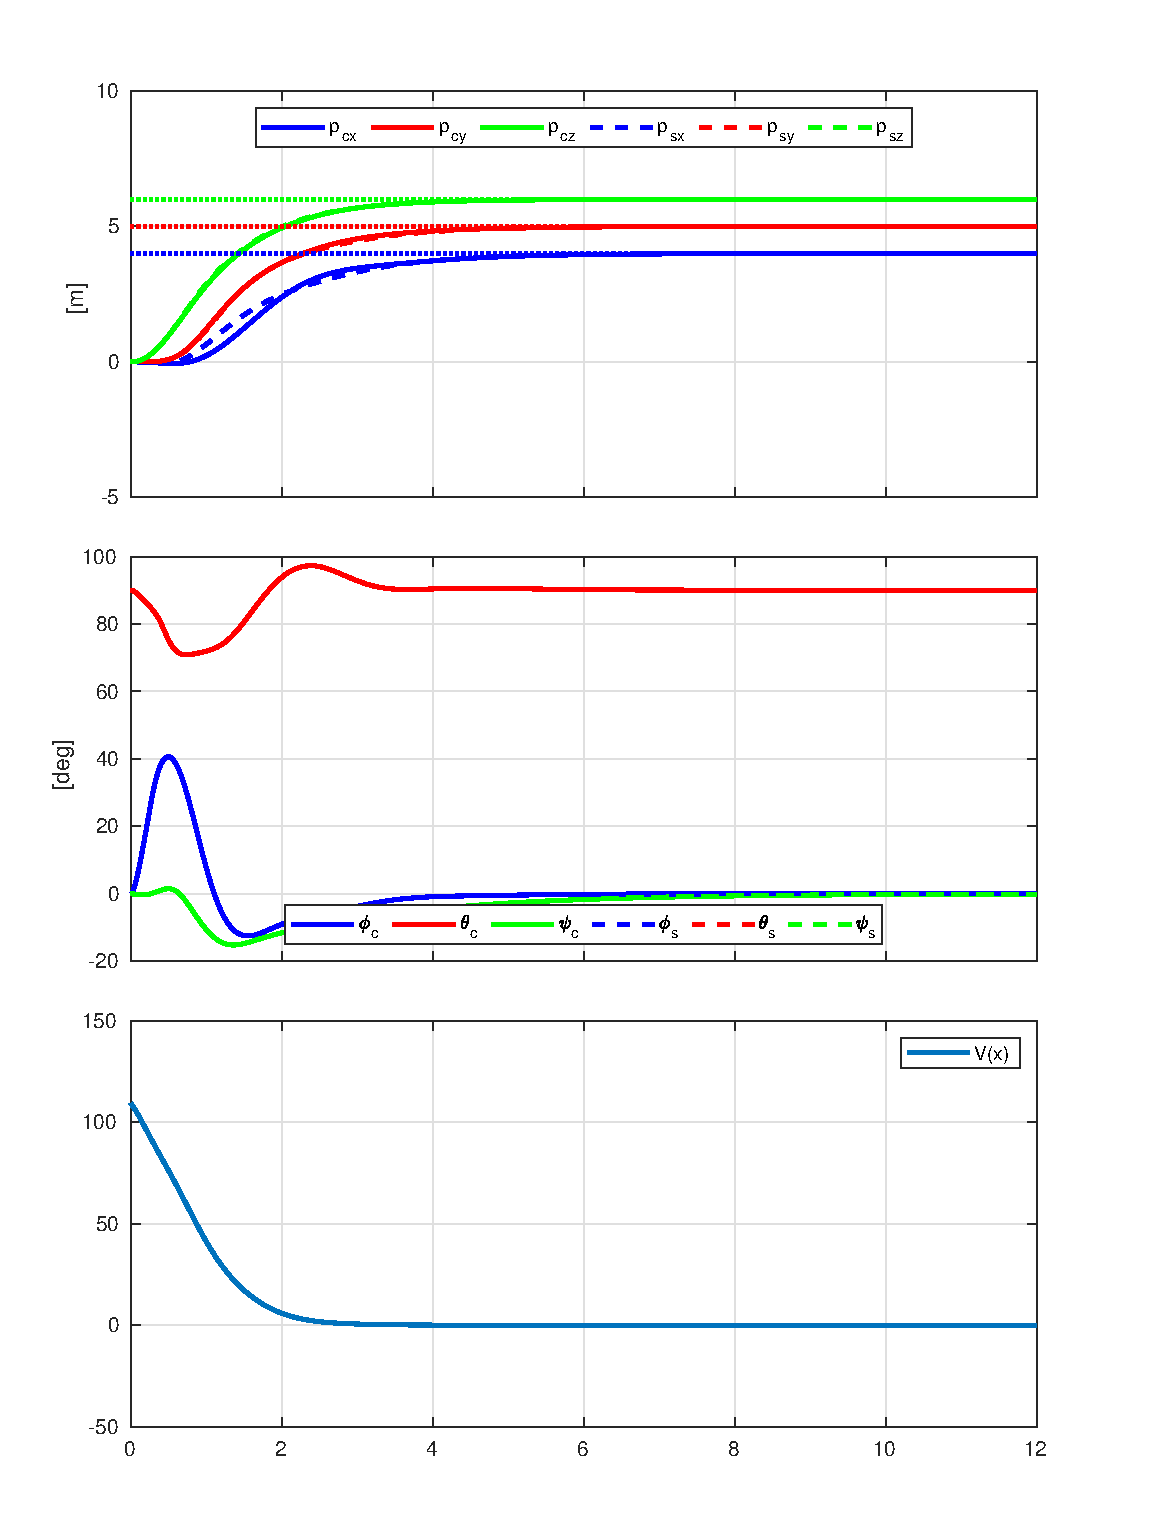
\includegraphics[trim=0cm 0.6cm 0cm 1cm,clip,width=1\columnwidth, height= 7cm]{figures/converge2.eps}
%     \vspace*{-5mm}
%     \caption{Simulation of the full model (solid) and \eqref{eq:dyna_simp} (dashed) with $\boldsymbol{u} = \boldsymbol{u}_{\text{lin}}$ as in 
%     \eqref{eq:u_lin} from an initial condition $\boldsymbol{\tilde x_0}$ within the basin of attraction.}
%     \label{fig_linearize_conv}
% \end{figure}
% Figure \ref{fig_linearize_conv} shows a simulation starting at the origin with a zero orientation on the three axes (horizontal UAV)
% and zero initial velocities,
% with a target position $\boldsymbol{p_{\text{eq}}} = [4,~5,~6]$ with a hovering stabilization (vertical UAV) with $\beta = 0$. The dotted line represents the target position on each axis. Note that the initial linear and angular velocities are zero.  The last graph shows the desirable exponential decay of $V$
% Figure \ref{fig_linearize_conv} shows both the simulation of the full model (solid) of \cite{sansou:stage} and of the simplified nonlinear model \eqref{eq:dyna_simp} (dashed) showing some significant differences in the initial response.
% When providing a larger target position $\boldsymbol{p_{\text{eq}}} =[8,~9,~10]$ (with the same orientation), the initial condition is outside the basin of attraction and diverging solutions are experienced as shown in Figure~\ref{fig_linearize_div}.
% \vspace*{-4mm}
% \begin{figure}[ht!]
%     \centering
%     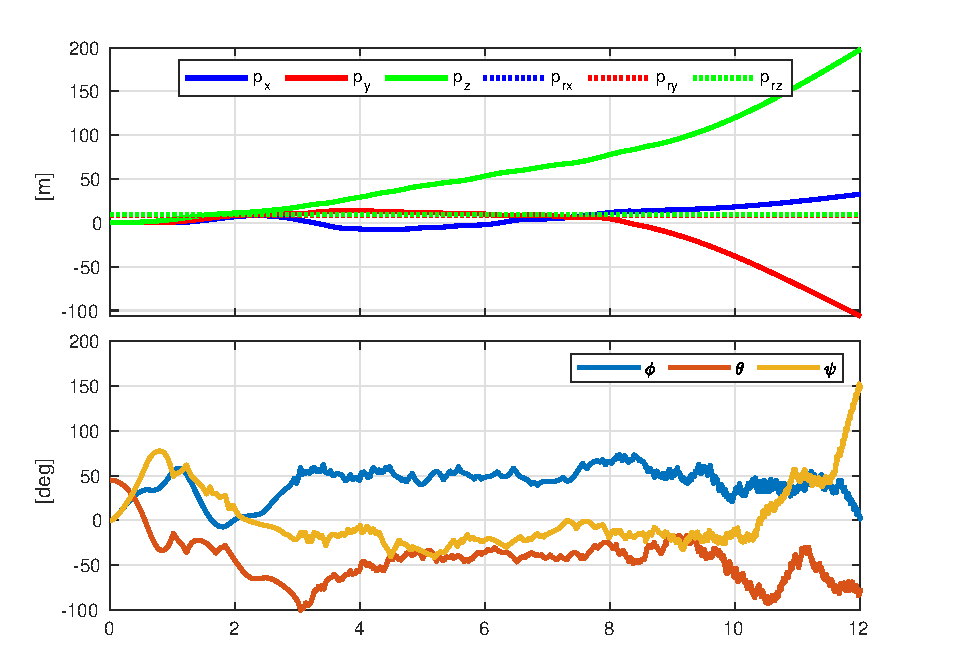
\includegraphics[trim=0cm 0cm 0cm 0cm,clip,width=\columnwidth, height=6cm]{figures/diverge2.eps}
%     \vspace*{-7mm}
%     \caption{Diverging simulation of the full model with $\boldsymbol{u} = \boldsymbol{u}_{\text{lin}}$ as in 
%     \eqref{eq:u_lin} from an initial condition $\boldsymbol{\tilde x_0}$ outside the basin of attraction.}
%     \label{fig_linearize_div}
% \end{figure}



% \subsection{Hysteresis-based local-global control design}
 
% Inspired by the local/global strategies presented in \cite[Ex. 1.7]{65}, similar to the solution presented in \cite{DBLP:conf/IEEEcca/AndreettoFZ16}, we use a hybrid mechanism to switch between the high performance local feedback \eqref{eq:u_lin} (as long as the state is in the basin of attraction of the equilibrium) and the less aggressive nonlinear controller \eqref{eq:u_nonlin}, which provides a larger region of attraction (and can be called with an abuse of notation the ``global controller''). To this end, we augment the controller state with a logical state variable

% $\ell \in \{0,1\}$, governing the choice of the control input 
% between \eqref{eq:u_nonlin} and \eqref{eq:u_lin} as
% \begin{align}
% \label{eq:u_hybrid}
%   \boldsymbol{u}=\boldsymbol{u}_{\text{hyb}} := \ell \boldsymbol{u}_{\text{nl}} + (1-\ell) \boldsymbol{u}_{\text{lin}},
% \end{align}
% We ensure, through the hybrid dynamics, that $\ell$ can only take values in $\{0,1\}$. 
% Its dynamics is defined by: 
% \begin{align*}
%     \left\{
%         \begin{array}{ll}
%             \dot \ell = 0,& \chi \in \mathcal{C}\\
%             \ell^{+} = 1-\ell,& \chi \in \mathcal{D}
%         \end{array}
%     \right.
% \end{align*}
% where $\chi = \left[\boldsymbol{p},~ \boldsymbol{v},~ \boldsymbol{q},~  \boldsymbol{\omega},~ l\right]$ is the complete closed loop state and $\mathcal{C}$ and $\mathcal{D}$ are, respectively, the flow and the jump sets, defined as
% \begin{align*}
%     & \mathcal{C} := \mathcal{C}_{0} \cup \mathcal{C}_{1}, ~ \mathcal{D} := \mathcal{D}_{0} \cup \mathcal{D}_{1},\\
%    & \mathcal{C}_{0} :=\{\boldsymbol{\chi} \in \mathbb{R}^{14}:~ V(\boldsymbol{\tilde x}) \le \overline{v} \mbox{ and } \ell=0\}\\
%    & \mathcal{C}_{1} :=\left\{\boldsymbol{\chi} \in \mathbb{R}^{14}:~ V(\boldsymbol{\tilde x}) \ge \underline{v} \mbox{ and } \ell=1 \right\}\\
%    & \mathcal{D}_{0} :=\left\{\boldsymbol{\chi} \in \mathbb{R}^{14}:~ V(\boldsymbol{\tilde x}) \geq \overline{v}\mbox{ and } \ell=0 \right\}\\
%    & \mathcal{D}_{1} :=\left\{\boldsymbol{\chi} \in \mathbb{R}^{14}:~ V(\boldsymbol{\tilde x}) \leq \underline{v}\mbox{ and } \ell=1 \right\}
% \end{align*}
% where $V(\boldsymbol{\tilde x}) := \boldsymbol{\tilde x}^\top S \boldsymbol{\tilde x}$  has been defined in the previous section, $\overline{v}=400$ has been determined in the previous section to satisfy \eqref{eq:Vdecrease},
%  and $\underline{v}$ is any positive constant satisfying $\underline{v}<\overline{v}$ (a smaller choice of $\underline{v}$ increases the hysteresis margin but postpones the desirable high performance tail of the feedback response). In our case we choose $\underline{v}= 350$.
% %
% The following result is an immediate consequence of the results in \cite[Ex. 1.7]{65} and the properties of our linear and nonlinear designs.

% \begin{proposition}
%   Under the action of the hybrid feedback \eqref{eq:u_hybrid}, the closed loop exhibits the same basin of attraction as the one associated with the nonlinear controller \eqref{eq:u_nonlin}, while always using the high-performance linear feedback \eqref{eq:u_lin} in the tail of the response.
% \end{proposition}

% We performed several simulations of the closed loop using the Matlab toolbox \cite{sanfelice_2017}. The simulations are carried out with the complete model of the UAV \cite{sansou:stage}, including all the nonlinear aerodynamic effects. A sample simulation is reported in Figure~\ref{fig_sim}, where we initialize the UAV at the origin with zero roll and yaw orientation, and with a pitch angle of 45 degrees. The target orientation is in the vertical hovering configuration and the target position is assigned to $\boldsymbol{p_{\text{eq}}} = [50,~25,~12.5]$.

% We observe that in the time phase $t \in \left[0,38\right]$, the UAV
% exhibits a graceful but slow convergence to the desired target position using the global controller ($\ell=1$). At that time, the state enters set $\mathcal{D}_1$ and the more aggressive local controller is activated up to the convergence to the desired equilibrium.

% To perform realistic simulations, the measurements are affected by 
% sensors noise. The intrinsic robustness of the hybrid feedback, established in \cite[Chapter 7]{65} is confirmed by the graceful performance degradation as a function of the amplitude of the measurement noise.

% \section{Schéma de commande hybride}

% \section{Simulations}






